


{\setbeamercolor{background canvas}{bg=tumgraylight}
	\begin{frame}[plain]
	\vfill
	\begin{center}
		\Huge\color{black}
		Engaging the ML community
		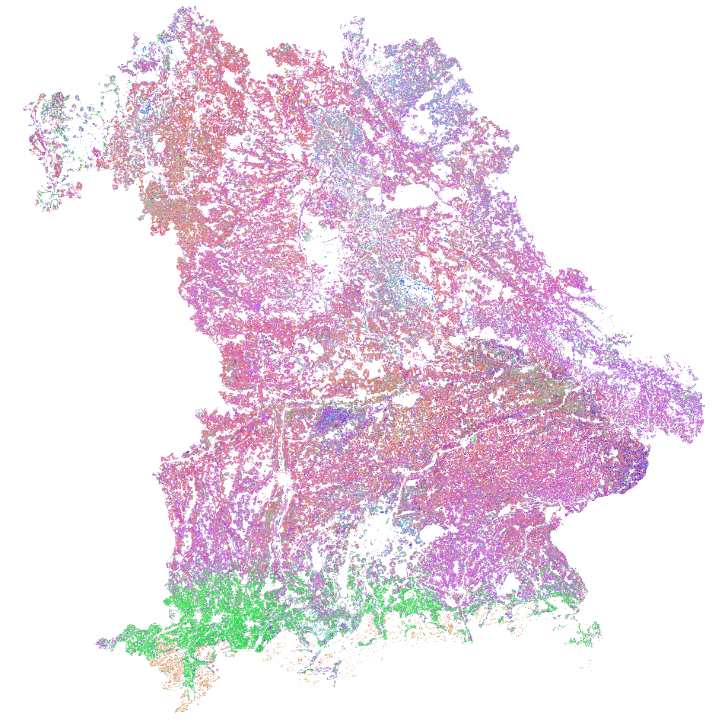
\includegraphics[width=7cm]{images/Bavaria}
		%		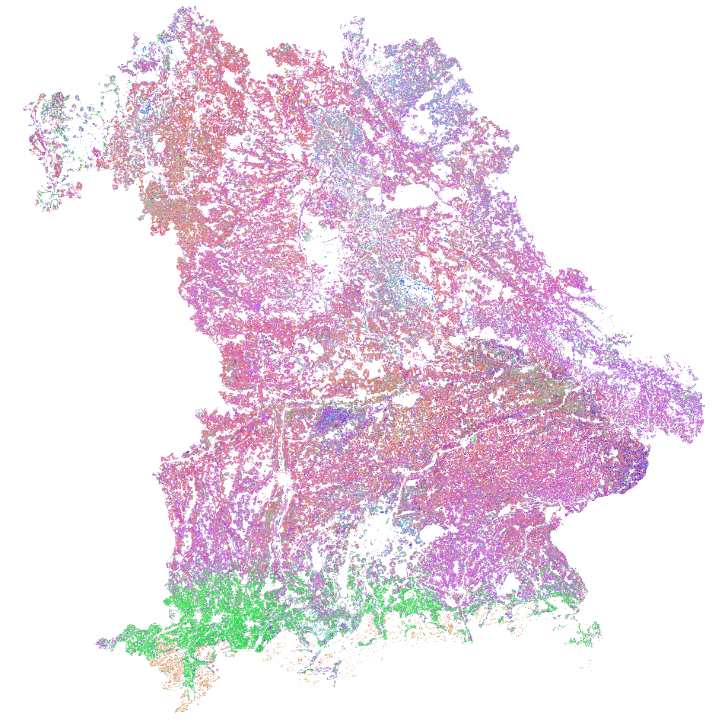
\includegraphics[width=4cm]{images/Bavaria}
	\end{center}
	
	\vfill
\end{frame}
}

\begin{frame}
\frametitle{Two Perspectives}
\centering

\begin{tikzpicture}[xscale=3.5, yscale=2]
%\draw[fill=tumblue, draw=none, opacity=0.5](-1,0) circle (1.5);
\node[fill=tumbluelight, draw=none, opacity=0.5, circle, minimum width=6cm, label=Earth Observation] at (-1,0){};

\node[fill=tumorange!50, draw=none, opacity=0.5, circle, minimum width=6cm, label=Machine Learning] at (1,0){};
%\draw[fill=tumorange, draw=none, opacity=0.5](1,0) circle (1.5);

%\node at (-1.3,1){Data};

\node[text width=3.5cm] at (-1,.9){\bluebf{method} is a \textbf{tool} for our \orangebf{data}};
\node[text width=3.5cm] at (1,.9){\orangebf{data} is a \textbf{benchmark} for our \bluebf{method}};


\node[text width=3.5cm] at (-1,.3){\bluebf{method} \textbf{should generalize} to applications of a specific sub-field};
\node[text width=3.5cm] at (1,.3){\bluebf{method} \textbf{must generalize} to many fields of applications};

\node[text width=3.5cm] at (-1,-.3){\orangebf{data} has specific \\ \textbf{phyisical properties}};
\node[text width=3.5cm] at (1,-.3){data is a \textbf{feature vector}};
%
%\node[text width=2cm] at (-1.3,-.6){{physics}, {sensors}, {applications}};

%\node at (1.3,1){Method};

%\node at (-1.3,1){IGARSS};
%\node at (-1.6,-1){ISPRS};
%\node at (-1.2,-.6){IEEE-GRSS};
%\node at (-1.8,.4){MDPI-RS Journal};
%\node at (-1.3,0){RSE Journal};
%
%\node at (1.3,1){NeurIPS};
%\node at (1.6,-1){CVPR};
%\node at (1.2,-.6){ICML};
%\node at (1.8,.4){ECCV};
%\node at (1.3,.2){ECML};
%
%\node at (0,.5){CVPR EarthVision};
%\node at (0,0){ECML MACLEAN};
%\node at (0,-.5){(ESA-$\Phi$-week)};

\end{tikzpicture}

\end{frame}


\begin{frame}
\frametitle{Common Datasets}
\centering
\begin{tikzpicture}[scale=2]
%\draw[fill=tumblue, draw=none, opacity=0.5](-1,0) circle (1.5);
\node[fill=tumbluelight, draw=none, opacity=0.5, circle, minimum width=6cm, label=Earth Observation] at (-.8,0){};

\node[fill=tumorange!50, draw=none, opacity=0.5, circle, minimum width=6cm, label=Machine Learning] at (.8,0){};
%\draw[fill=tumorange, draw=none, opacity=0.5](1,0) circle (1.5);

\node[font=\Large\bfseries, text width=2cm] at (0,0) {Common Datasets};

\end{tikzpicture}
\end{frame}


\begin{frame}
\frametitle{Building Large-Scale Crop Type Mapping Datasets}

\begin{columns}
	
	\column{.5\textwidth}
	
	\Large
	
	\begin{description}\setlength\itemsep{1em}
		\item[\color{tumblue}collected] yearly within European \textbf{Common Agricultural Policy} (CAP)
		\item[\color{tumblue}declared] by Farmers at \textbf{crop subsidy} applications
		\item[\color{tumblue}today] slowly made publicly available (on a national basis by French 
\includegraphics[height=.9em]{images/IGN-logo}, Bavarian Stmelf 
\includegraphics[height=.9em]{images/stmelf-logo}, etc.)
		\item[\color{tumblue}in future] further harmonized within \textbf{Europe's INSPIRE} directive (correct?)
	\end{description}
	
	\column{.5\textwidth}
	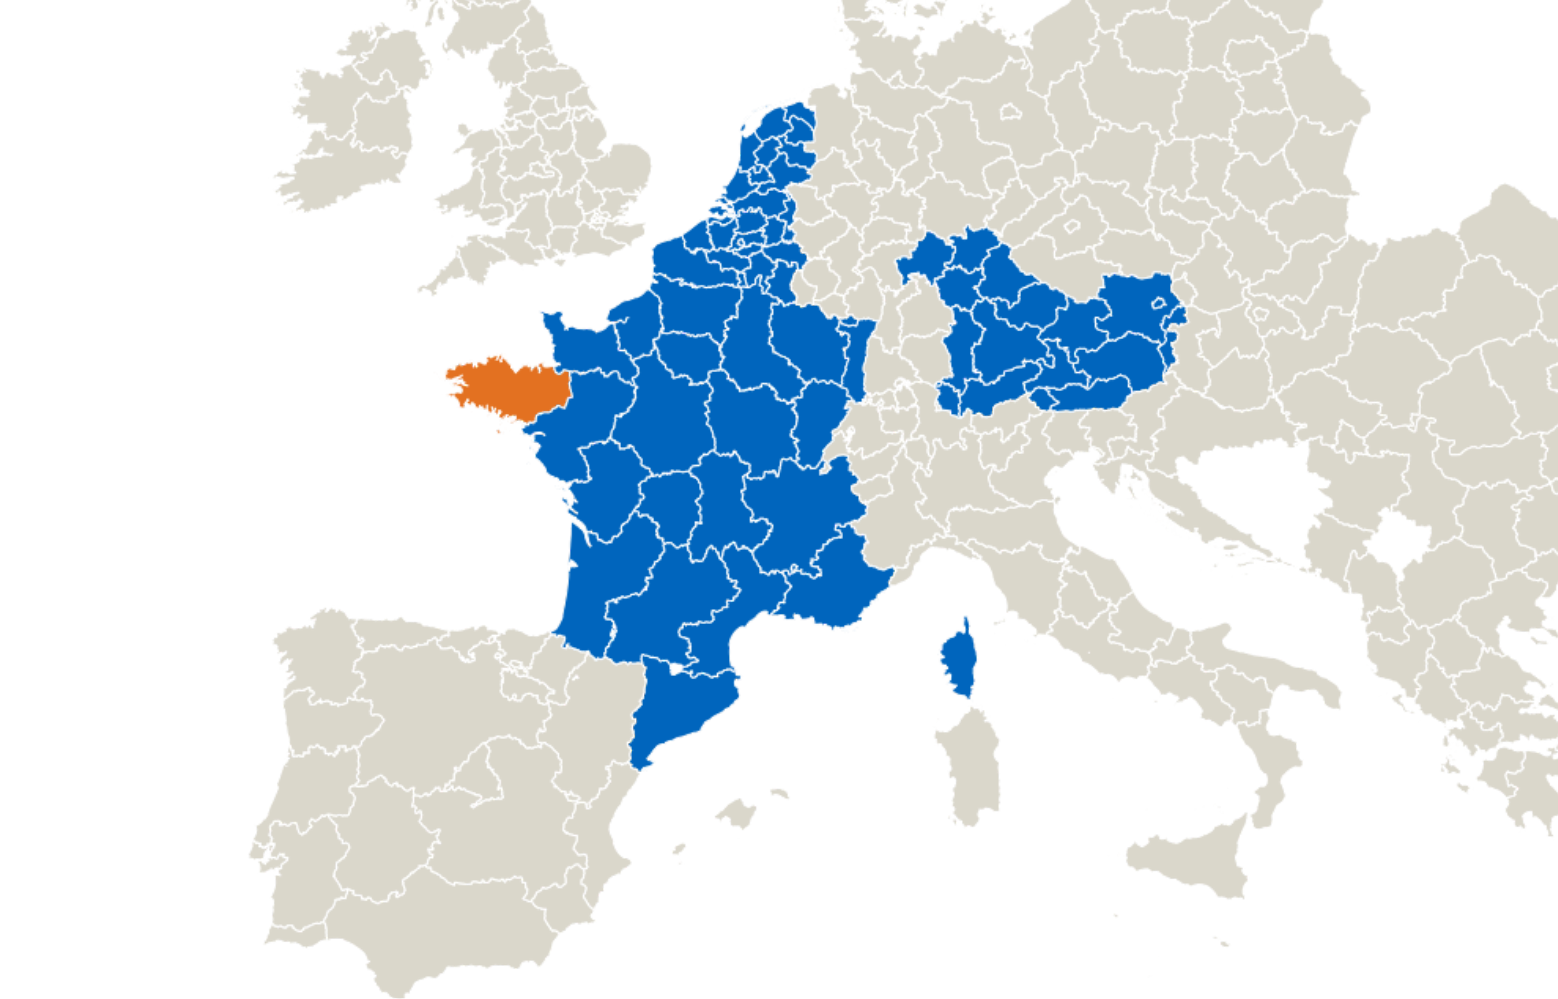
\includegraphics[width=\textwidth]{images/europe_data2}
	
	
	
	
\end{columns}

\vspace{2em}


\end{frame}


\begin{frame}
\frametitle{BreizhCrops Dataset (ICML Workshop Submission)}

\begin{center}
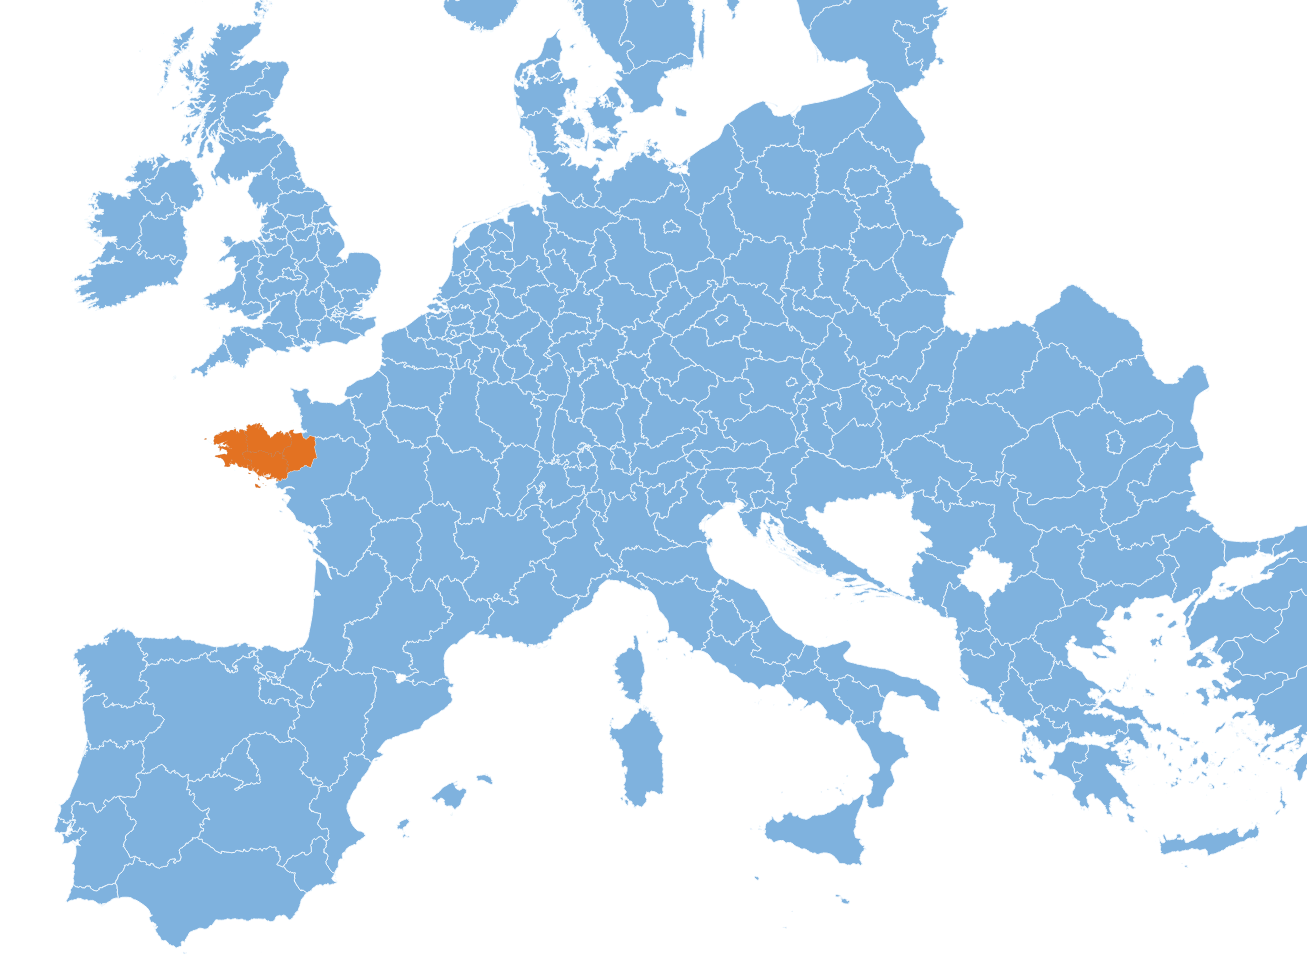
\includegraphics[width=3cm]{images/map/europe}
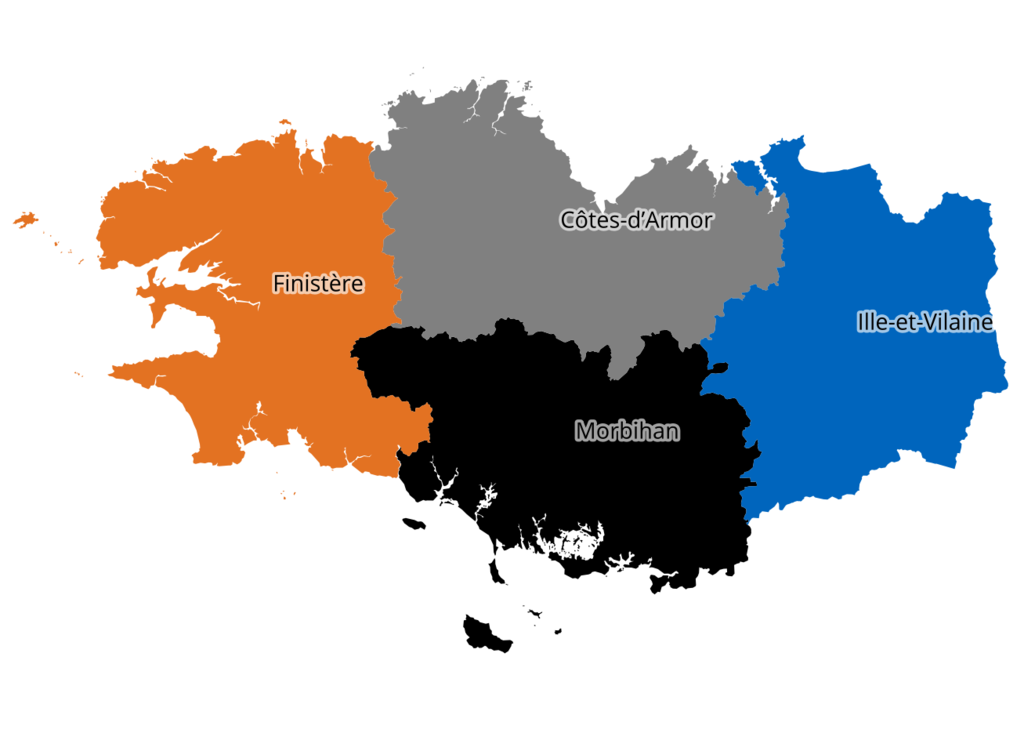
\includegraphics[width=3cm]{images/map/regions}
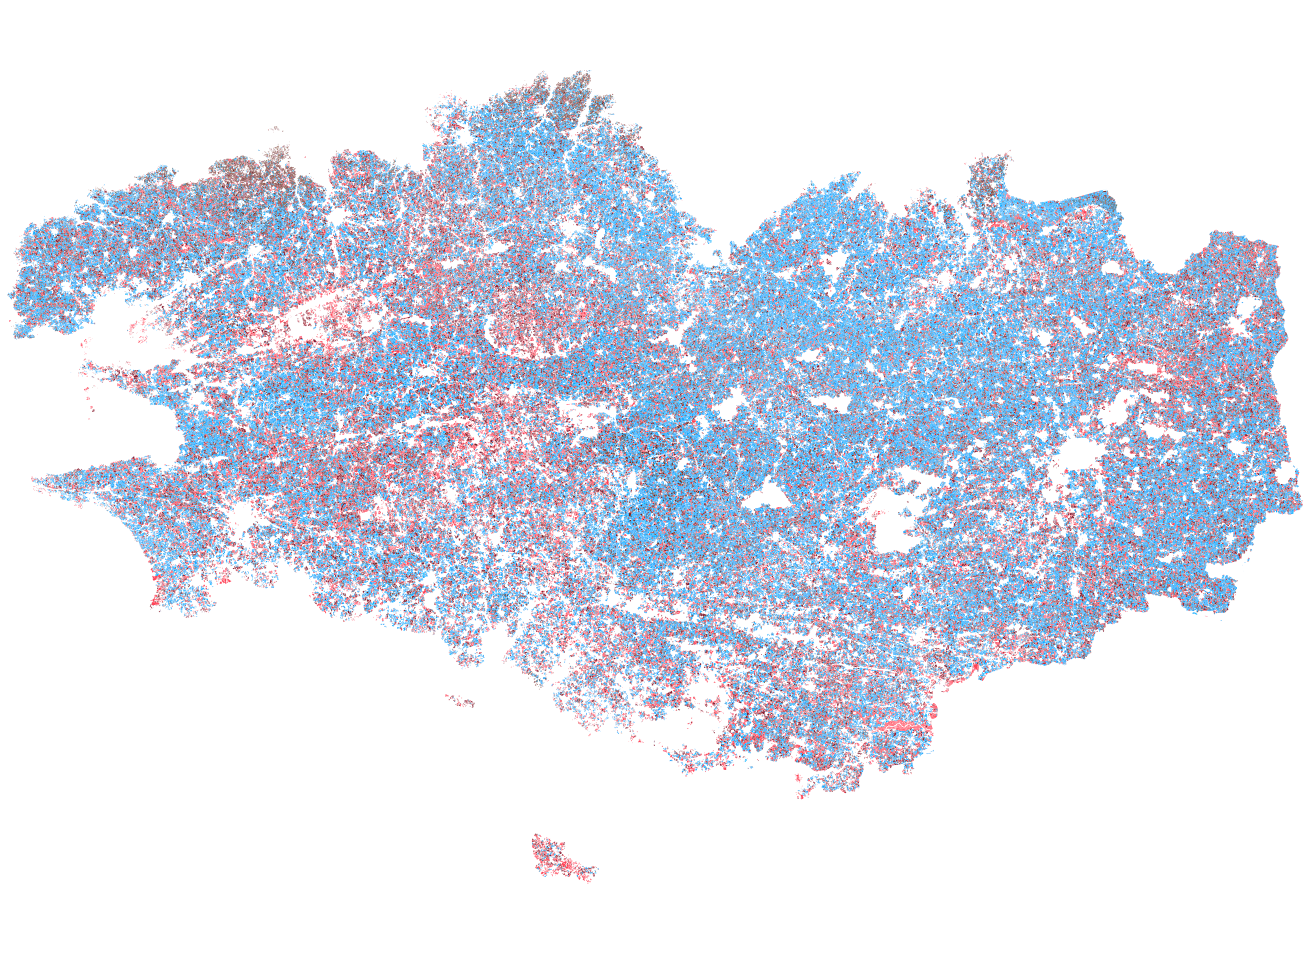
\includegraphics[width=3cm]{images/map/breizh}
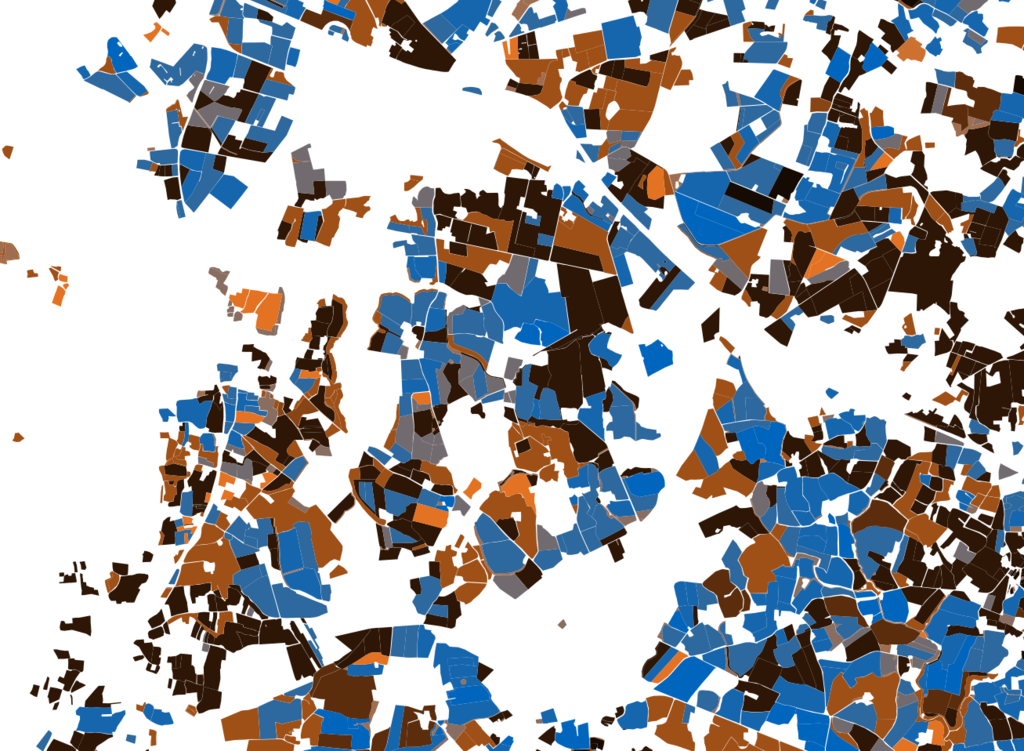
\includegraphics[width=3cm]{images/map/parcels}
\end{center}

%\vspace{1em}

%\tikzsetnextfilename{example}

\newcommand{\dataexample}[1]{
	
	
	


\begin{tikzpicture}
	
	\tikzstyle{annot} = [font=\tiny\sffamily, text=tumblue]
	\tikzstyle{point} = [thin, tumbluelight, shorten >= .25em, shorten <= .25em]
	
	% from /home/marc/projects/EV2019/images/example/tstop.txt
	\def\tstopv{0.6285714285714286}
	\def\class{winter barley}
	
	\begin{groupplot}[
	group style={
		group name=my plots,
		group size=1 by 1,
		columns=1,
		xlabels at=edge bottom,
		xticklabels at=edge bottom,
		vertical sep=1em,
	},
	date coordinates in=x,
	date ZERO=2017-01-01,
	xmin=2017-01-01,
	xmax=2017-12-31,
	ylabel near ticks,
	ylabel style={font=\sffamily\small, rotate=-90},
	width=\textwidth,
	height=3cm,
	axis x line=bottom,
	axis y line=left,
%	enlarge x limits=0.01,
	xtick={2017-01-01,2017-05-01,2017-08-01,2017-12-01},
	xticklabels={January,April,August,December},
	ymajorgrids,
    ymax=10000
	]
	
\nextgroupplot[thin,
%	smooth=1pt,
no marks,  
ylabel={},
draw opacity=.8,
%		tension=0.001,
legend columns=2,
%y tick label style={rotate=90},
legend style={at={(.5,1)},anchor=south, line width=1pt, fill=tumblue!10}
]

\addplot[b1color] table [x=doa, y=B1, col sep=comma, forget plot] {#1};
\addplot[b9color] table [x=doa, y=B9, col sep=comma, forget plot] {#1};
\addplot[b10color] table [x=doa, y=B10, col sep=comma] {#1};

\addplot[b11color] table [x=doa, y=B11, col sep=comma, forget plot] {#1};
\addplot[b12color] table [x=doa, y=B12, col sep=comma] {#1};

\addplot[b5color] table [x=doa, y=B5, col sep=comma, forget plot] {#1};
\addplot[b6color] table [x=doa, y=B6, col sep=comma, forget plot] {#1};
\addplot[b7color] table [x=doa, y=B7, col sep=comma, forget plot] {#1};
\addplot[b8color] table [x=doa, y=B8, col sep=comma, forget plot] {#1};
\addplot[b8Acolor] table [x=doa, y=B8A, col sep=comma] {#1};

\addplot[b2color] table [x=doa, y=B2, col sep=comma, forget plot] {#1};
\addplot[b3color] table [x=doa, y=B3, col sep=comma, forget plot] {#1};
\addplot[b4color] table [x=doa, y=B4, col sep=comma] {#1};
	
%	\draw [red, very thick, ->] ([xshift=5em]plt.north west) -- ([xshift=5em]plt.south west) node [midway, rotate=90, fill=white, yshift=2pt] {faster} ;
%	\node(glab) at (10em,0.5) {ground (signal)};
	
%	\sample{images/example/3685593.csv}
%	
%	\sample{images/example/6053223.csv}
%	\draw[fill=white, draw=none, opacity=.5] (axis cs:\tstopv,0) rectangle (axis cs:1,1.1);
	
%	\node[annot](cllab) at (axis cs:.2,1.3) {clouds (noise)};
%	\draw[point] (cllab) -- (axis cs:.13,.7);
%	\draw[point] (cllab) -- (axis cs:.25,.7);
%	\draw[point] (cllab) -- (axis cs:.53,1);
%	\draw[point] (cllab) -- (axis cs:.45,.85);
%	
%	\node[annot](glab) at (axis cs:.8,1.3) {ground (signal)};
%	\draw[point] (glab) -- (axis cs:.38,.3);
%	\draw[point] (glab) -- (axis cs:.21,.3);
%	\draw[point] (glab) -- (axis cs:.7,.3);
%	
%	\draw (axis cs:\tstopv,0) -- (axis cs:\tstopv,1) node[above]{$\tstop$};
%	
%	
%	
%	\legend{3 atmospheric, 2 short-wave infrared, 5 near infrared, 3 visible bands}
%	
		\end{groupplot}
	
	\end{tikzpicture}
	
}
\begin{columns}
	\column{.5\textwidth}
	
	\textbf{corn grain and silage}
	\dataexample{images/breizhcrops/example/6139251.csv}
	
	\column{.5\textwidth}
	
	\textbf{temporary meadows}
	\dataexample{images/breizhcrops/example/3685593.csv}
	
\end{columns}

%\vspace{1em}


\begin{columns}
	\column{.5\textwidth}
	
	580k samples of Time Series $\M{X}$ and labels $\V{y}$. \Large \url{https://github.com/TUM-LMF/BreizhCrops}
	
	\column{.5\textwidth}
	
	\small\raggedright
	\textsl{
		Rußwurm M., Lefèvre S., and Körner M (2019). \textbf{BreizhCrops: A Satellite Time Series Dataset for Crop Type Identification}. ICML 2019 Time Series Workshop. arXiv:1905.11893
	}
	
\end{columns}

\end{frame}

\begin{frame}
	\frametitle{Challenges and Impact}
	
	\Large
	
	\begin{columns}[t]
	
	\column{.5\textwidth}
	
	\visible<1->{
		\Large\textbf{Impact}
		\vspace{1em}
		
		\begin{description}[itemsep=.5em]
		\item large scale \bluebf{real-world dataset}
		\item effectively \bluebf{unlimited data} (spatially and temporally)
		\item \bluebf{assessing generalization} over large regions
		\item extraction for further \bluebf{vegetation characteristics} in future work (drought indicator, early classification, crop yield)
		\end{description}
	}
	
	\column{.5\textwidth}
	
	\visible<2->{
	\Large\textbf{Challenges}
	\vspace{1em}
	
	\begin{description}[itemsep=.5em]
		\item \bluebf{imbalanced} class \bluebf{labels}
		\item classes with \bluebf{similar characteristics}
		\item non-Gaussian noise induced by \bluebf{clouds}
		\item \bluebf{regional} \bluebf{variations} in the class distributions
		\item \bluebf{spatial} \bluebf{autocorrelation}
		\item \bluebf{irregular} temporal \bluebf{sampling} distance
		\item \bluebf{variable} \bluebf{sequence} length
	\end{description}
}
	

	\end{columns}

\setcounter{framenumber}{35}
	
\end{frame}


